\documentclass{article}
\usepackage[utf8]{inputenc}
\usepackage{graphicx}
\graphicspath{ {~/Downloads/hw4/build/CodeBlocks/} }
\usepackage{url}
% For basic math, align, fonts, etc.
\usepackage{amsmath}
\usepackage{amsthm}
\usepackage{amssymb}
\usepackage{mathtools}
\usepackage{mathrsfs}
\mathtoolsset{showonlyrefs}

\usepackage{hyperref} 
% For color
\usepackage{xcolor}
\definecolor{dark-red}{rgb}{0.4,0.15,0.15}
\definecolor{dark-blue}{rgb}{0,0,0.7}
\hypersetup{
    colorlinks, linkcolor={dark-blue},
    citecolor={dark-blue}, urlcolor={dark-blue}
}
\begin{document}
\begin{center}
    \begin{Large}
    CMPSCI 687 Project
    \end{Large}
    \\
    By: Arpit Singh
\end{center}

\noindent {\bf \\ \\ Brief description of INAC and What it does: } \\ \\Incremental Natural Actor Critic (INAC) algorithm is a variant of Actor Critic algorithm in which the weight vector w is used which is incrementally updated and used as an estimate of the natural gradient to update the actor weights. \\ \\
In the actor critic algorithm, the actor stores the policy while the critic critiques the actions chosen by the actor by computing the corresponding value function. \\ \\
The state values are estimated by calculation of $v^T \phi(s) $. The critic weights v are updated with TD($\lambda$) after which the policy weights $\theta$ of the actor are updated based on the TD error $\delta$ and the eligibility trace $e^{\theta}$. In INAC algorithm, we introduce weight vectors w also that get incrementally updated. They are used for estimating the natural gradient in order to update the actor weights $\theta$. \\ \\
The algorithm uses the natural gradient $G(u)^{-1}  \triangledown_u J(\pi) $ where G(u) is the Fisher information matrix.
\\\\
\noindent {\bf Pseudocode: } \\ \\
1: Choose a according to $ \pi (a|s) $. \\ 
2: Take action a in s, observe s' and r. \\
3: $\delta$ = r+$\gamma v^T \phi(s')$-$v^T \phi(s) $ \\
4: $e^v$=$\gamma \lambda e^v$+ $\phi(s)$ \\
5: v=v+$\alpha_{critic}  \delta  e^v $ \\
6: $e^{\theta}$=$\gamma \lambda e^{\theta}$ + $dlnpi(\phi(s),a)$ \\
7: w=w-$( \alpha_{critic} * dlnpi(\phi(s),a) * dlnpi(\phi(s),a)^T * w)$+ $( \alpha_{critic} * \delta * e^{\theta} ) $ \\
8: $\theta$ = $\theta$ + $\alpha_{actor} w $ \\ \\
\noindent Also, for terminal states, everything is same as above except: \\
1: $\delta$ = r-$v^T \phi(s) $ \\
2: $e^v$, w and $e^{\theta}$ are set to zero. \\ \\
\noindent {\bf Tuning of hyperparameters and Results on MDPs: } \\ \\
I tuned the hyperparameters for the domains Cart Pole and Acrobot. A brief description of how I tuned them for each domain is mentioned in their respective sections.
\\\\
Following are the MDPs on which the algorithm was applied: 
\\\\
\noindent 1. Cart Pole: \\
The hyperparameters are: \\
fourier basis order: 4 \\
alpha(actor): 0.001 \\
alpha(critic): 0.002 \\
lambda: 0.65 \\
gamma: 0.9 \\
number of trials: 110 \\
number of episodes per trial: 370 \\ \\
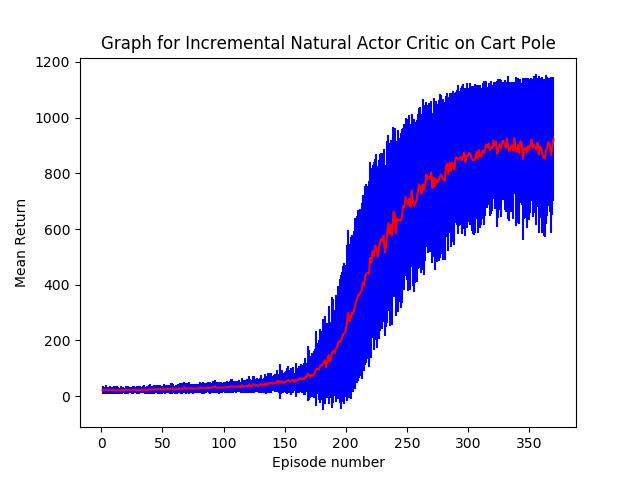
\includegraphics[width=12cm]{cartpole} \\ \\
Tuning the hyperparameters: I tried to keep alpha(actor) and alpha(critic) closer to each other on seeing the improvements in the results. $\lambda$ was decreased from 1 so the agent learns from not too many previous states. $gamma$ was slightly decreased and set to 0.9 to discount the obtained rewards. Fourier basis order was increased to 4. I saw that it was not learning quickly in the initial episodes so I set the number of episodes to a large value (370 episodes) after which it started learning properly which can also be seen in the above graph. \\ \\
\noindent 2. Acrobot: \\ 
The hyperparameters are: \\
fourier basis order: 4 \\
alpha(actor): 0.001 \\
alpha(critic): 0.001 \\
lambda: 0.15 \\
gamma: 1 \\
number of trials: 110 \\ 
number of episodes per trial: 150 \\ \\
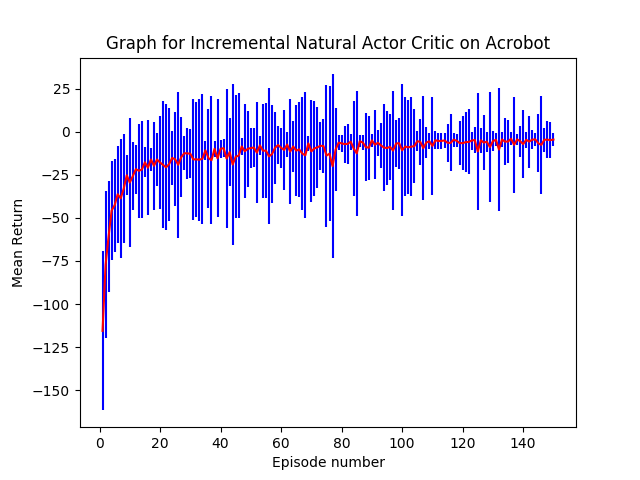
\includegraphics[width=12cm]{acrobot} \\ \\
Tuning the hyperparameters: $\lambda$ was decreased to a smaller value so the agent learns from only a few previous states. I kept alpha(actor) and alpha(critic) closer to each other on seeing the improvements in the results. $gamma$ was set to 1 as we do not want to discount the rewards (since the movements help in adding energy to create the desired torque and we don't want to discourage the agent) and Fourier basis order was increased to 4. I saw that it learnt very quickly so I set the number of episodes to 150 episodes which was sufficient enough. \\ \\
\noindent {\bf References: } \\ \\
1. \url{http://ieeexplore.ieee.org/stamp/stamp.jsp?tp=&arnumber=6315022&isnumber=6314593}

\end{document}
